\documentclass[8pt, handout=show,notes=show]{beamer}

\usepackage{fontspec}
%Ligatures={Contextual, Common, Historical, Rare, Discretionary}
\setmainfont[Mapping=tex-text]{Linux Libertine O}

%%%lua off
%\usepackage[utf8x]{inputenc}
%\usepackage[T1]{fontenc} 
%\usepackage{lmodern}

\usepackage{graphicx}
\usepackage[french,ruled,vlined]{algorithm2e}
\usepackage[authoryear,round]{natbib}
\usepackage[frenchb]{babel}

\usepackage{default}
\usetheme[width=2cm]{Goettingen}
\usecolortheme{rose}

% \usepackage[colorlinks=true,urlcolor=blue,citecolor=green,linkcolor=blue,bookmarks=true]{hyperref}
\author[]{Simon Carrignon \\ 
\vfill Directeurs : Frédéric Bouchard \& Stephane Schmitt }
\institute[]{
	Université Paris 7 Denis Diderot\\
	\pgfdeclareimage[height=0.5cm]{ephe}{images/logo_p7_large.jpg} %declare logo image with an alias here 

}

\usepackage[small]{caption}
\useoutertheme{infolines}
\usepackage{subfigure}
\usepackage[footheight=1em]{beamerthemeboxes}

\addfootboxtemplate{\color{black}}{\color{white}
\hspace{2em}Simon Carrignon \hfill\insertframenumber/\inserttotalframenumber\hspace{2em}\null}

\title{La Robotique \'Evolutionnaire comme modèle pour étudier la Théorie de l'\'Evolution}

\usepackage[]{natbib}
\bibpunct{[}{]}{,}{a}{,}{,}
\date{9 Septembre 2013}

\begin{document}


\begin{frame}
	\maketitle
\end{frame}


	%%%----------------------------------------------------------------------
	%%%----------------------------------------------------------------------
\section{Avant Propos}
\begin{frame}{Avant Propos}
	Pourquoi ce mémoire? 
	\vfill
	\begin{columns}
		\column{.5\textwidth}
		Des théories biologiques:
		\begin{figure}[hbp]
			\begin{center}
				\includegraphics<1>[width=4cm]{images/reponse.png}
			\end{center}
		\end{figure}
		(cours de génét. des pop., génét. quant., L2)
		\column{.5\textwidth}
		Des résultats en informatique:
		\begin{figure}[hbp]
			\begin{center}
				\includegraphics<2>[width=3cm]{images/sample.png}
			\end{center}
		\end{figure}
		(cours d'IA, L3)
	\end{columns}
\end{frame}

\begin{frame}{Avant Propos}
	Un dialogue renouvelé et approfondi à travers la \emph{Robotique \'Evolutionnaire}.
	\begin{itemize}
		\item Des problématiques communes
		\item Des méthodes communes
	\end{itemize}
	\begin{figure}[hbp]
		\begin{center}
			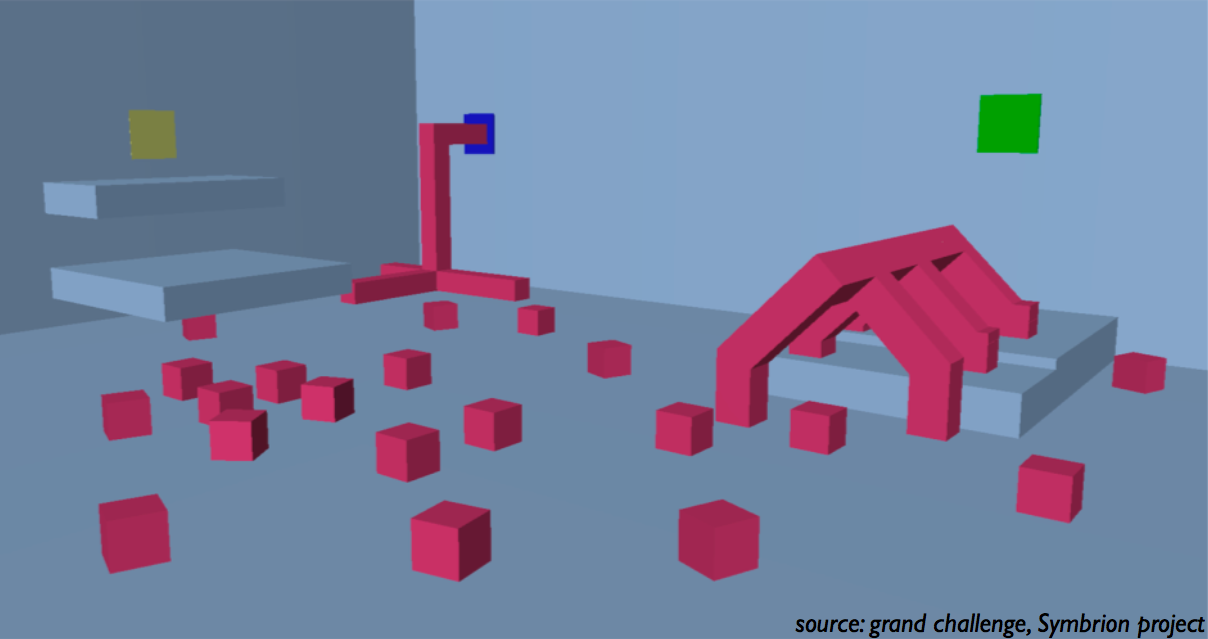
\includegraphics[width=4cm]{images/symbrion-gc1b.png} \\
			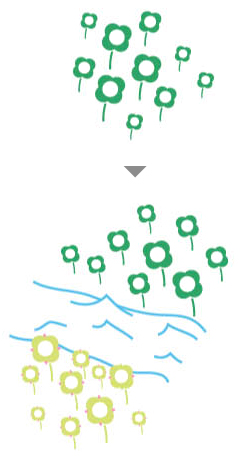
\includegraphics[width=1.2cm]{images/SpeciationAl.jpg}
			\hspace{1cm} 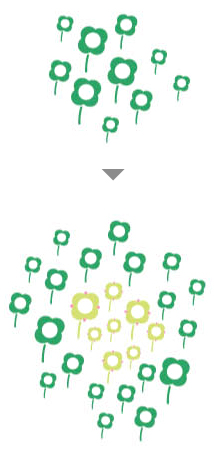
\includegraphics[width=1.2cm]{images/SpeciationSy.jpg}
		\end{center}
	\end{figure}
\end{frame}

\begin{frame}{Sommaire}
		Justifier l'utilisation de la Robotique \'Evolutionnaire pour étudier la théorie de l'\'Evolution.
		\vfill
	\begin{enumerate}
		\item La Théorie de l'\'Evolution.
		\item Les outils pour l'étudier.
		\item La Robotique \'Evolutionnaire.
	\end{enumerate}
\end{frame}
	%%%------------------------------------------------------------------------
	%%%----------------------------------------------------------------------

	%%%----------------------------------------------------------------------
	%%%----------------------------------------------------------------------
\section{La Théorie de l'évolution}

\subsection{Histoire et Structure}
\begin{frame}{La théorie darwinienne de l'évolution}
	Chez \cite{darwin1859originspeciesbymeansnaturalselectionorpreservationfavouredracesstrugglelife}:
	\begin{quote}
		Theory of descent with modification by variation and Natural Selection
	\end{quote}

	\vfill

	D'après \cite{gayon1991darwinetlapresdarwin}, deux composantes :
	\begin{itemize}
		\item Descente avec Modification : variation aléatoire et hérédité.
		\item L'Hypothèse de la sélection naturelle : ``survival of the fittest'' (formulation de Spencer).
	\end{itemize}
	\vfill
	Conséquences : une théorie qui explique comment les espèces se modifient \emph{et} se différencient.
\end{frame}

\begin{frame}{Darwin}
	Nous avons donc deux éléments qui structurent la théorie de l'évolution selon Darwin.
	\vfill
	\begin{alertblock}{Mais des problèmes se posent :}

		\begin{itemize}
			\item Descente avec Modification : théorie hérédité  qui n'existe pas et critique Jenkin
			\item SN : impossible à ``prouver''
		\end{itemize}
	\end{alertblock}
\end{frame}


\begin{frame}{Des Biométriciens à la Synthèse Moderne}
	Après de Darwin: tentatives de résoudre les précédents problèmes et d'articuler la biologie autour de la vision darwienne.
	\vfill

	\begin{enumerate}
		\item Les Biometriciens : ``preuve'' empirique de l'action de la SN
		\item Les Mendéliens : théorie génétique mendélienne en contradiction avec les hypothèses darwiniennes.
	\end{enumerate}
	\begin{columns}
		\column{.5\textwidth}
		\begin{figure}[h]
			\begin{center}
				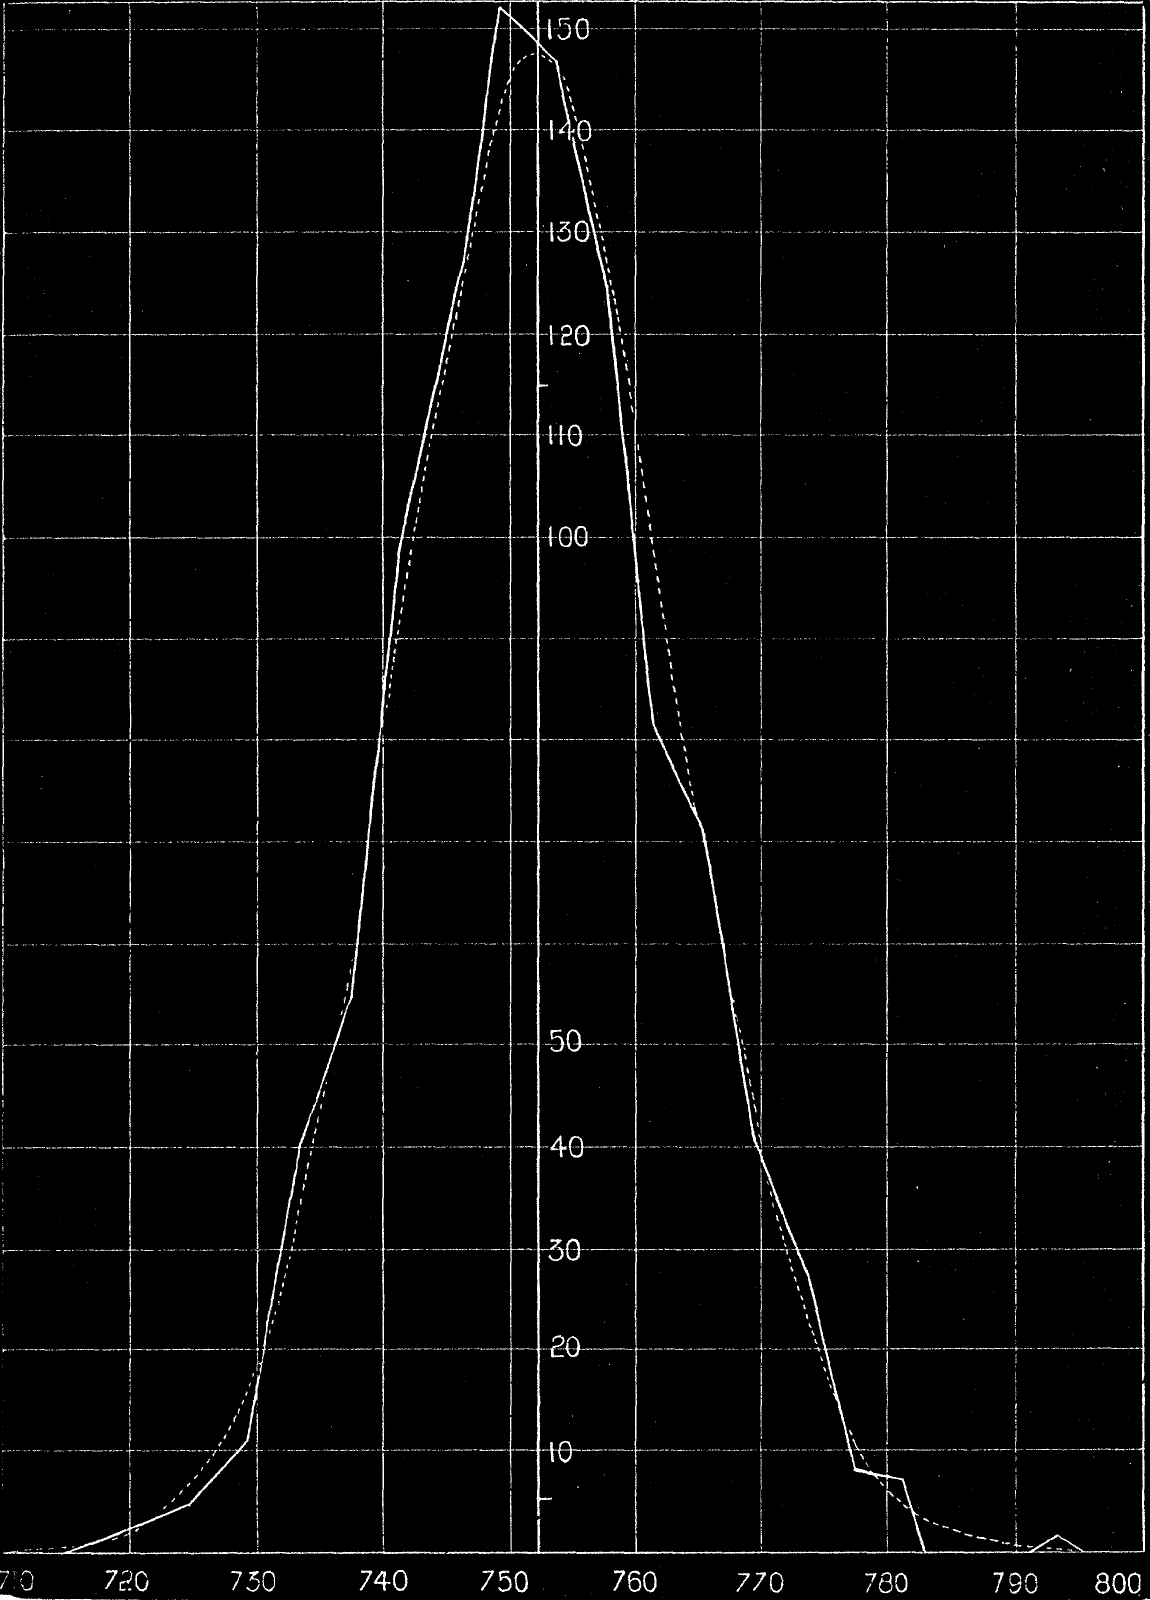
\includegraphics[width=.5\textwidth]{images/gauss1.png}
			\end{center}
			\caption{\cite{weldon1893certaincorrelatedvariationsincrangonvulgaris}}
		\end{figure}
		\column{.5\textwidth}
		\begin{table}
			\begin{tabular}{c|cc}
				Parents & L & r \\\hline
				L & LL & Lr \\
				r & Lr & rr \\
			\end{tabular}
			\caption{Hybridation de caractères mendéliens.}
		\end{table}
	\end{columns}

	\vfill

	Puis, Fisher, Haldane, Wright, les architectes de la génétique des populations et la \emph{Synthèse Moderne}.

\end{frame}
\begin{frame}{Théorie synthétique de l'évolution}
	Synthèse Moderne :
	\vfill
	\begin{itemize}
		\item	Les individus biologiques sont le produit de l'information génétique transmise par les gamètes (Weismann et dogme central):
			\begin{center}
				ADN$\rightarrow$transcription$\rightarrow$traduction$\rightarrow$protéine
			\end{center}
		\item L'information génétique et transmise de $G^-$ en $G^-$ via l'ADN et varie aléatoirement.
		\item L'évolution correspond à des changements de fréquences alléliques.
	\end{itemize}
	\vfill
	Vision de l'évolution directement reprise et appliquée ``aveuglement'' en AE et RE : nécessité de bien la comprendre, son histoire, les choix faits\dots
\end{frame}
\begin{frame}{Débats et visions actuelles}
	\'Etudier certains débats (par ex. les unités de sélection) permet :

	\begin{itemize}
		\item illustrer limites et nuances,
		\item dégager des visions alternatives.
	\end{itemize}

	\vfill
	Une vision actuelle pour concilier nombreux points de TSE et approches divergentes : vision de PGS.
	\begin{figure}[h]
		\begin{center}
			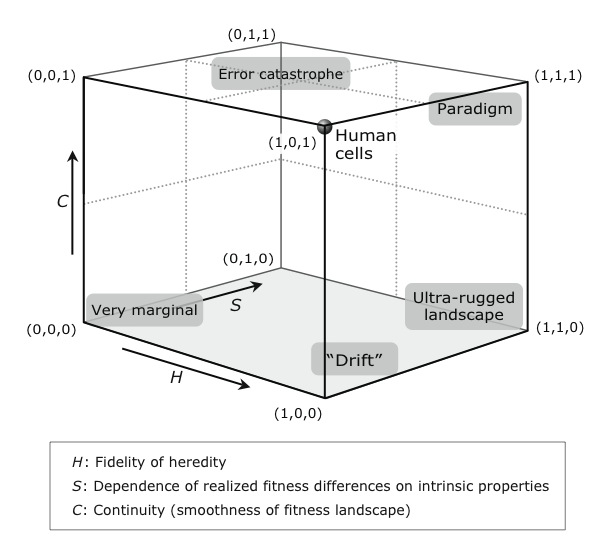
\includegraphics[width=4cm]{./images/PGS.png}
			\caption{extrait de \citet[p.~64]{godfrey2009darwinian}}
		\end{center}
	\end{figure}
\end{frame}

	%%%----------------------------------------------------------------------
	%%%----------------------------------------------------------------------
\section{Méthodes d'études}
	%%%----------------------------------------------------------------------
	%%%----------------------------------------------------------------------

	%%%----------------------------------------------------------------------
	%%%----------------------------------------------------------------------
\begin{frame}{Méthodes d'études}
	Quelles méthodes existent? 
	\begin{enumerate}
		\item Sélection Artificielle \& Modèles expérimentaux 
		\item Expériences de pensée
		\item Modèles théorique \&  simulation
	\end{enumerate}
	\vfill

	\begin{exampleblock}{Remarque}
		Il ne s'agit pas d'une recherche exhaustive mais sélection de méthodes :
		\begin{itemize}
			\item largement utilisées et reconnues,
			\item qui partagent des points essentiels avec la RE.
		\end{itemize}
	\end{exampleblock}
\end{frame}
\subsection{Sélection Artificielle \& Modèles expérimentaux}
\begin{frame}{Sélection Artificielle \& Modèles expérimentaux}
	Amener l'évolution dans le laboratoire:
	\begin{enumerate}
		\item Darwin avec la SA des éleveurs.
		\item Morgan \& Dobzhansky avec les Drosophiles.
		\item \cite{lenski94dynamicsadaptationdiversification10000generationexperimentbacterialpopulations} avec E. Coli.
	\end{enumerate}
	\vfill
	\begin{alertblock}{Problèmes}
		\begin{itemize}
			\item \'Echelles temporelles,
			\item Limitations à certains organismes vivants très particuliers,
			\item\ldots
		\end{itemize}

	\end{alertblock}

\end{frame}

\subsection{Les expériences de pensée}
\begin{frame}{Les expériences de pensée}
	Imaginer une situation particulière pour comprendre un problème : pas de limite sur le type d'EV, pas de restrictions expérimentales\dots
	\vfill
	\begin{alertblock}{Problèmes}
		\begin{itemize}
			\item Aucun lien avec données empiriques.
			\item Nombreux paramètres mis de côté
			\item Aprioris et biais introduits inconsciemment\ldots
		\end{itemize}
	\end{alertblock}
	\vfill
	$\rightarrow$ Même les plus critiques s'accordent sur la valeur, au moins suggestive, des expériences de pensée.
\end{frame}

\subsection{Modèles théoriques \& Simulation}
\begin{frame}{Modèles théoriques \& Simulation}
	Nouvelles approches de la science (Vue sémantique des théories, V. Frassen, Suppes,\dots) qui s'articulent mieux avec la biologie de l'évolution.
	\vfill

	Construction de modèles artificiels (informatiques) pour étudier la biologie (cf Vie Artificielle)

	\begin{block}{Avantages}
		\begin{itemize}
			\item Simulation de VA comme : ``\emph{Opaque Though Experiment}''
				\begin{itemize}
					\item Grande Liberté,
					\item Contourne les problèmes liées à étude sur être vivants.
				\end{itemize}
			\item études de systèmes complexes,
			\item plus de puissance que les expériences de pensées,
			\item finesse de conception et d'analyse des resultats,
			\item \dots
		\end{itemize}

	\end{block}

	\vfill
	
	Lien avec la biologie parfois difficiles (notamment pour \emph{alife}) et connexions empiriques nécessaires.

\end{frame}
	%%%----------------------------------------------------------------------
	%%%----------------------------------------------------------------------


	%%%----------------------------------------------------------------------
	%%%----------------------------------------------------------------------
\section{La Robotique \'Evolutionnaire}
\subsection{Histoire \& Méthode}
\begin{frame}{Algorithmique \'Evolutionnaire et Robotique}

	\vfill
	\begin{columns}
		\column{.5\textwidth}
		\begin{figure}[h]
			\begin{center}
				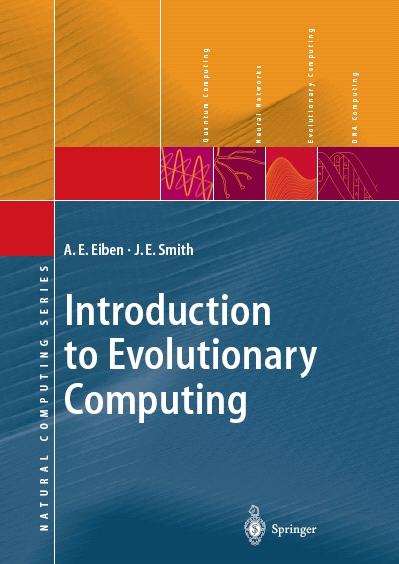
\includegraphics[height=4cm]{images/ec}
			\end{center}
			\caption{\cite{eiben03introductiontoevolutionarycomputing}}
			\label{fig:ec}
		\end{figure} 

		\vfill
		Algoritmique Évolutionaire 1970 : \cite{holland75adaptationnaturalartificialsystem}


		\column{.5\textwidth}

		\begin{figure}[h]
			\begin{center}
				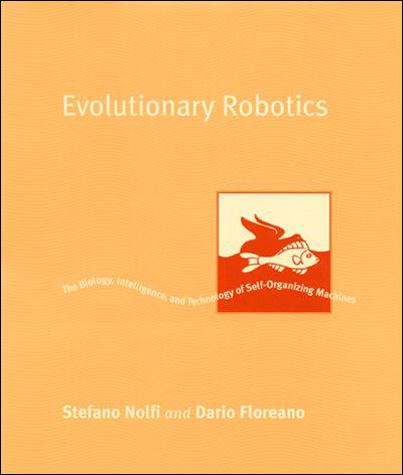
\includegraphics[height=4cm]{images/er}
			\end{center}
			\caption{\cite{nolfi00evolrobobiolintetechselfmach}}
			\label{fig:er}
		\end{figure}

		\vfill
		Robotique Évolutionnaire 1990 : \cite{nolfi00evolrobobiolintetechselfmach}
	\end{columns}
	\vfill

	$\rightarrow$ utiliser Darwin pour concevoir des systèmes artificiels
\end{frame}

\begin{frame}{Algorithme Classique}
	\begin{algorithm}[H]
		\dontprintsemicolon 
		\caption{Un Algorithme classique de Robotique \'Evolutionnaire}\label{alg:RE}
		Définition de la tâche \;
		Choix des contrôleurs \;
		Initialisation de la génération G0 \;
		\While{Expérimentateur \neq satisfait}{
			Test des contrôleurs \;
			Calcul de la fitness \;
			Sélection \;
			Reproduction (mutations,croisements) \& création d'une nouvelle génération \;
		}
	\end{algorithm}

	\vfill
	\begin{figure}[h]
		\begin{center}
			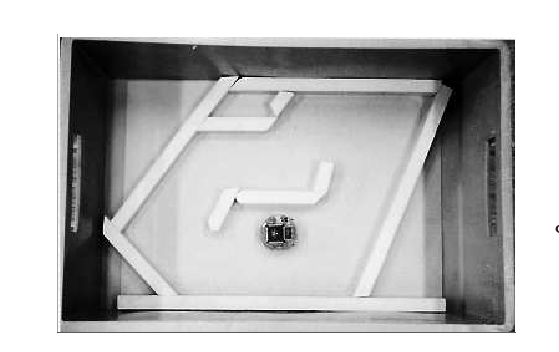
\includegraphics[width=5cm]{images/oldERfloreano.png}
		\end{center}
		\caption{Floreano 90}
	\end{figure}
	\vfill
	Problèmes pratiques et théoriques (lenteur, optimisation via fitness)


\end{frame}
\subsection{Approches \emph{Open Ended}}
\begin{frame}{Approches \emph{Open Ended} non dirigées}

	Objectif:
	\begin{itemize}
		\item surmonter les problèmes de ER traditionnelle.
	\end{itemize}

	Solution :
	\begin{itemize}
		\item rapprochement avec la biologie.
	\end{itemize}

	\vfill

	\begin{description}
		\item[Approche \emph{open ended} :] pas de but à l'évolution, étude de l'évolution en elle même,
			\begin{center}
				et,\\
			\end{center}
		\item[\'Evolution \emph{non dirigée} :] eviter au maximum l'introduction de critères ``objectifs''(qui mobilisent une connaissance extérieur) de sélection.
	\end{description}


	
\end{frame}

\begin{frame}{Robotique \& Biologie}
	Lier Robotique et Biologie via l'approche de PGS.
	\vfill

	Exemple:
	\begin{columns}
		\column{.5\textwidth}
		\begin{figure}[h]
			\begin{center}
				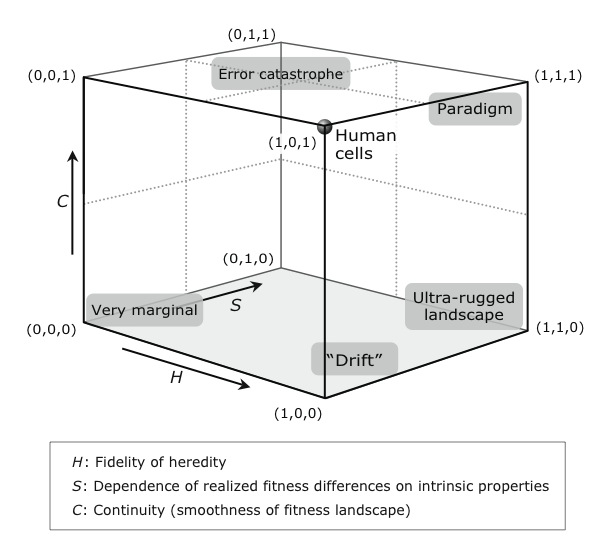
\includegraphics[width=4cm]{./images/PGS.png}
			\end{center}
			\caption{extrait de \citet[p.~64]{godfrey2009darwinian}}
		\end{figure}
		\column{.5\textwidth}
		\begin{figure}[h]
			\begin{center}
				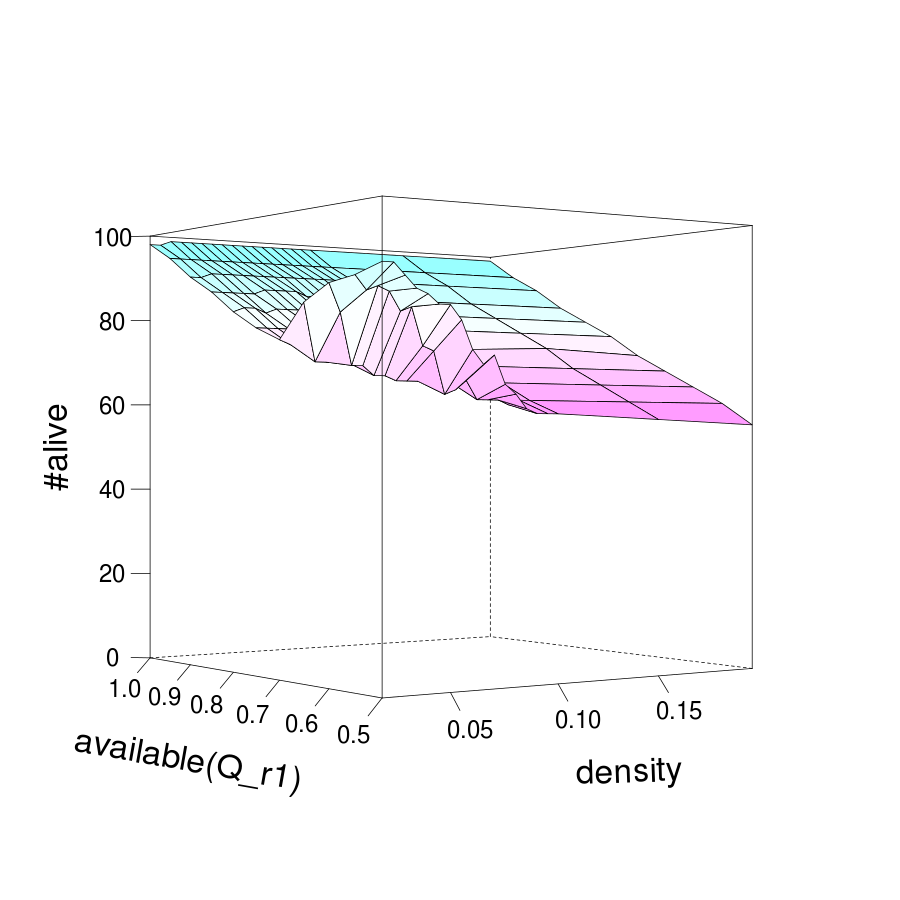
\includegraphics[width=5cm]{/home/simon/projects/TAO/evorob/Perso/Simon/doc/20111122-Specialisation-Density-Heatmap/images/active_median}
			\end{center}
			\caption{Travail mémoire de master EPHE avec N. Bredèche}
		\end{figure}
	\end{columns}

\end{frame}


	%%%----------------------------------------------------------------------
	%%%----------------------------------------------------------------------



\section{Conclusion}

\begin{frame}{Robotique \'Evolutionnaire et Biologie, un échange à double sens}
	\begin{itemize}
		\item concepts fondamentaux et théoriques doivent être discutés pour que les transferts Bio $\rightarrow$ Info soient fructueux.
			\vfill
		\item RE : candidate idéale pour explorer ces théories et fournir des éclairages différents (Robot $\rightarrow$ Bio).
	\end{itemize}

\end{frame}

	%%%----------------------------------------------------------------------
	%%%----------------------------------------------------------------------


\bibliographystyle{apalike}
\bibliography{/home/simon/Documents/biblio/memoireLophiss}
\end{document}




